\documentclass[pdftex,twocolumn,10pt,letterpaper]{extarticle}

%%% Set these variables appropriately
%%%
%% Note:  Authors is hardcoded below, this line only used for the PDF info
\newcommand{\AUTHORS}{Sol Boucher, Anuj Kalia, David G. Andersen, and Michael Kaminsky}
\newcommand{\TITLE}{Lightweight Preemptible Functions}
\newcommand{\KEYWORDS}{TODO}
\newcommand{\CONFERENCE}{USENIX ATC '20}
\newcommand{\PAGENUMBERS}{no}       % "yes" or "no"
\newcommand{\COLOR}{yes}
\newcommand{\showComments}{yes}
\newcommand{\showThesis}{no}
\newcommand{\comment}[1]{}
\newcommand{\onlyAbstract}{no}

%%%%%%%%%%%%%%%%%%%%%%%%%%%%%%%%%%%%%%%%%%%%%%%%%%%%%%%%%%%%%%%%%%%%%


%%%
%%%  Fonts
%%%
\usepackage[T1]{fontenc}
\usepackage[utf8]{inputenc}
\usepackage{libertine}
\usepackage[libertine]{newtxmath}
\usepackage{inconsolata}
\usepackage{textcomp}
\usepackage[mathcal]{euscript}

%%%
%%%  Page Setup
%%%
\special{papersize=8.5in,11in}
\setlength{\pdfpagewidth}{8.5in}
\setlength{\pdfpageheight}{11in}

\usepackage{ifthen}
\ifthenelse{\equal{\PAGENUMBERS}{yes}}{%
\usepackage[nohead,
            left=1in,right=1in,top=1in,
            footskip=0.5in,bottom=1in,     % Room for page numbers
            columnsep=0.25in
            ]{geometry}
}{%
\usepackage[noheadfoot,left=1in,right=1in,top=1in,
            footskip=0.5in,bottom=1in,
            columnsep=0.25in
	    ]{geometry}
}

%%%
%%%  Captions
%%%
\usepackage[font=bf]{caption}
\usepackage{subcaption}

%%%
%%% Source code
%%%
\usepackage{xcolor}
\definecolor{commentgreen}{RGB}{2,112,10}
\usepackage{listings}
\lstset{language=C++,
        tabsize=4,
        basicstyle=\small\ttfamily,
        keywordstyle=\color{blue}\ttfamily,
        breaklines=true,
        commentstyle=\color{commentgreen}\ttfamily,
        captionpos=b,
        columns=flexible
}

\lstset{emph = {linger_t, u64, cont_t},
        emphstyle = {\color{blue}}}

%%  Space between figure and caption (assuming caption
%%  is below figure)
%\usepackage[font=bf,aboveskip=0pt]{caption} % SPACE
%%  Space between caption and body text of document
%\addtolength{\textfloatsep}{-7pt} % SPACE

%%%
%%%  Section headings
%%%
\usepackage{titlesec}
%\titlespacing{\paragraph}{0pt}{*1}{*1}      % SPACE
%\usepackage[compact]{titlesec}              % SPACE

%\titleformat{\section}%                     % ACM: caps + period (for 10pt doc)
%  {\bf\large\uppercase}{\thesection.\quad}{0pt}{}

%%% The following should mimic the 9pt ACM sig-alt style headings
%%%
%\titleformat{name=\section}%                 % ACM: caps + period (for 9pt doc)
%  {\bf\LARGE\uppercase}{\thesection.\quad}{0pt}{}
%\titleformat{name=\section,numberless}%      % ACM: for categores, etc.
%  {\bf\LARGE}{}{0pt}{}[\vspace*{-2pt}]
%\titleformat{\subsection}%                   % ACM
%  {\bf\LARGE}{\thesubsection\quad}{0pt}{}
%\titleformat{\subsubsection}%                % ACM
%  {\it\Large}{\thesubsubsection\quad}{0pt}{}

%%%
%%%  Lists
%%%
\usepackage{enumitem}
\setlist{itemsep=0pt,parsep=0pt}             % more compact lists

%%%
%%%  Header / Footer
%%%
\usepackage{fancyhdr}
\renewcommand{\headrulewidth}{0pt}

\ifthenelse{\equal{\PAGENUMBERS}{yes}}{%
  \pagestyle{plain}
}{%
  \pagestyle{empty}
}

%%%
%%%  Bibliography
%%%
\usepackage[numbers]{natbib}

%%%
%%%  Footnotes / Endnotes
%%%
\interfootnotelinepenalty=10000  % Split footnotes are annoying

% If you want endnodes, uncomment:
%\usepackage{endnotes}
%\usepackage{drafthead}
%\let\footnote=\endnote

%%%
%%%  Tables
%%%
\usepackage{booktabs}
\usepackage{color}
\usepackage{colortbl}
\usepackage{float}                           % Must appear before hyperref to
                                             % avoid weird PDF compile issues

%%%
%%%  PDF setup
%%%
\ifthenelse{\equal{\COLOR}{yes}}{%
  \usepackage[colorlinks,citecolor=blue]{hyperref}%         % for online version
}{%
  \usepackage[pdfborder={0 0 0}]{hyperref}%  % for paper (B&W) version
}
\usepackage{url}

\hypersetup{%
pdfauthor = {\AUTHORS},
pdftitle = {\TITLE},
pdfsubject = {\CONFERENCE},
pdfkeywords = {\KEYWORDS},
bookmarksopen = {true}
}

% Anonymize figure inclusion
% Requires pdfTeX version 1.40.17
\pdftrailerid{} %Remove ID
\pdfsuppressptexinfo15 %Suppress PTEX.Fullbanner and info of imported PDFs

% Uncomment next line if your printer outputs black
% boxes instead of drop shadows; older PDF interpreters
% in printers can't handle those PDF 1.5 features
%\pdfminorversion=3
%\pdfobjcompresslevel=2


%%
%% Figure placeholder macros
%%

\definecolor{placeholderbg}{rgb}{0.85,0.85,0.85}
\newcommand{\placeholder}[1]{%
\fcolorbox{black}{placeholderbg}{\parbox[top][1.5in][c]{0.95\columnwidth}{#1}}}


%%%
%%%  Misc
%%%
\usepackage[pdftex]{graphicx}
\usepackage{soul}
% this allows \st and friends to work with citations
\soulregister\cite7
\soulregister\ref7
\soulregister\pageref7

%\setlength{\parindent}{0pt}
%\setlength{\parskip}{\baselineskip}

%\clubpenalty=10000  % Don't allow orphans
%\widowpenalty=10000 % Don't allow widows

%%%
%%%  To appear/appeared in text on title page
%%%
\usepackage[absolute]{textpos}
\newcommand{\ToAppear}{%
\begin{textblock*}{\textwidth}(0.95in,0.4in)
\begin{flushright}
    %\noindent{\fbox{\textsf{Under submission---please do not redistribute.}}}
    %  --OR--
    \noindent{\small To appear in \textit{Proceedings of the XYZ}\\
    \noindent{\small \textit{Conference (XYZ'08)}, City, State, Month 2008}}
    %  --OR--
    %\noindent{\small In \textit{Proceedings of the XYZ}\\
    %\noindent{\small \textit{Conference (XYZ'08)}, City, State, Month 2008}}
\end{flushright}
\end{textblock*}
}

%%%
%%%  Sample ACM Copyright Block
%%%
\newfloat{acmcr}{b}{acmcr}
\newcommand{\AcmCopyright}{%
\begin{acmcr}
\parbox[b]{20pc}{%
\footnotesize
Permission to make digital or hard copies of all or part of this work
for personal or classroom use is granted without fee provided that
copies are not made or distributed for profit or commercial advantage
and that copies bear this notice and the full citation on the first
page.  To copy otherwise, to republish, to post on servers or to
redistribute to lists, requires prior specific permission and/or a fee.

{\em Conference}, Month Date--Date, Year, Location\\
Copyright 200X ACM X-XXXXX-XX-X/XX/XX ...\$5.00}
\end{acmcr}}

%%%
%%%  Comments
%%%
\newcommand{\note}[2]{
    \ifthenelse{\equal{\showComments}{yes}}{\textcolor{#1}{#2}}{}
}

% Change these to your own initials as you like...
\newcommand{\solb}[1]{\note{magenta}{SOLB: #1}}
\newcommand{\akalia}[1]{\note{red}{AKALIA: #1}}
\newcommand{\dga}[1]{\note{green}{DGA: #1}}
\newcommand{\mk}[1]{\note{blue}{MK: #1}}
\newcommand{\thesis}[1]{\ifthenelse{\equal{\showThesis}{yes}}{\note{violet}{THESIS: #1}}{}}

\date{}
\title{\textbf{\TITLE}\vspace{-0.75em}}
\author{{\large Sol Boucher\footnotemark\addtocounter{footnote}{0}, Anuj Kalia\thanks{This author was at Carnegie Mellon during this project.}, David G.\@ Andersen\footnotemark[1], and Michael Kaminsky\footnote{This author was \textit{not} at Carnegie Mellon during this project.}~~\footnotemark[1]}\\
{\normalsize \em \footnotemark[1]~Carnegie Mellon University \; \footnotemark[2]~~Microsoft Research \; \footnotemark[3]~~BrdgAI}\vspace{-0.75em}}

% This needs to be the last thing before \begin{document}
%\usepackage{microtype}  % SPACE

%%%%%%%%%%%%%%%%%%%%  START DOCUMENT  %%%%%%%%%%%%%%%%%%%%%%%%
\begin{document}

\maketitle

\ifthenelse{\equal{\PAGENUMBERS}{yes}}{%
  \thispagestyle{fancy}
}{%
  \thispagestyle{empty}
}

%\AcmCopyright
%\ToAppear

We introduce novel programming abstractions for isolation of both time and memory.
They operate at finer granularity than traditional primitives, supporting preemption
at sub-millisecond timescales and tasks defined at the level of a function call.
This resolution enables new functionality for application programmers, including
users of unmanaged systems programming languages, all without requiring changes to
the existing systems stack.  Despite being concurrency abstractions, they employ
synchronous invocation to allow application programmers to make their own scheduling
decisions.  However, we found that they compose naturally with existing concurrency
abstractions centered around asynchronous background work, such as threads and
futures.  We demonstrated how such composition can enable asynchronous cancellation
of
threads and the implementation of preemptive thread libraries in userland, both
regarded for decades as challenging problems.

\ifthenelse{\equal{\onlyAbstract}{no}}{%
\section{Introduction}
\label{sec:intro}

As the scope and scale of Internet services continues to grow, system designers
have sought platforms that simplify scaling and deployment.
Services that outgrew self-hosted servers moved to datacenter racks, then
eventually to virtualized cloud hosting environments.
However, this model only partially delivered two related benefits:
\begin{enumerate}
\item Pay for only what you use at very fine granularity
\item Scale up rapidly on demand
\end{enumerate}

\noindent
The VM approach suffered from relatively coarse granularity:  Its atomic compute unit
of machines were billed at a minimum of minutes to months.  Relatively long startup
times often required system designers to keep some spare capacity online to handle
load spikes.

These shortcomings led cloud providers to introduce a new model, known as
serverless computing, in which the customer provides \textit{only} their code,
without having to configure its environment.   Such ``function as a service''
(FaaS) platforms are now available as AWS Lambda~\cite{www-amazon-lambda}, Google
Cloud Functions~\cite{www-google-cf}, Azure Functions~\cite{www-microsoft-af}, and
Apache OpenWhisk~\cite{www-apache-openwhisk}.  These platforms provide a model in
which: (1)  user code is invoked whenever some event occurs (e.g., an HTTP
API request), runs to completion, and nominally stops running (and being
billed) after it completes; and (2)  there is no state preserved between
separate invocations of the user code.  Property (2) enables easy auto-scaling
of the function as load changes.

Because these services execute within a cloud provider's
infrastructure, they benefit from low-latency access to other cloud
services.  In fact, acting as an access-control proxy is a recurring microservice
pattern:\@ receive an API request from a user, validate it, then access
a backend storage service (e.g., S3) using the service's credentials.

In this paper, we explore a design intended to reduce the tension between two of
the desiderata for cloud functions:\@ low latency invocation and low cost.  Contemporary
invocation techniques exhibit high latency with a
large tail; this is
unsuitable for many modern distributed systems which involve
high-fanout communication, sometimes performing thousands of
lookups to handle each user request.  Because user-visible response time often
depends on the tail latency of the slowest chain of dependent
responses~\cite{Dean:cacm2013}, shrinking the tail is crucial~\cite{Jalaparti:sigcomm2013,
Xu:nsdi2013,Li:socc2014,Jeon:asplos2016}.

Thus we seek to reduce the invocation latency and improve predictability, a
goal supported by the impressively low network latencies available in modern
datacenters. For example, it now takes $<20\mu{}s$ to perform an RPC between two
machines in
Microsoft Azure's virtual machines~\cite{Firestone:nsdi2018}. We believe,
however, that fully leveraging this improving network performance will require
reducing microservices' invocation latencies to the point where the network is
once again the bottleneck.

We further hypothesize---admittedly without much proof for this chicken-and-egg
scenario---that substantially reducing both the latency and cost of running
intermittently-used services will enable new classes and scales of applications
for cloud functions, and in the remainder of this paper, present a design that
achieves this.  As Lampson noted, there is power in making systems 
``fast rather than general or powerful''~\cite{Lampson1983}, because fast
building blocks can be used more widely.

Of course, a microservice is only as fast as the slowest service it relies on;
however, recall that many such services are offered in the same clouds and
datacenters as serverless platforms. Decreasing network latencies will push
these services to respond faster as well, and new stable storage
technologies such as 3D XPoint (projected to offer sub-microsecond reads and
writes) will further accelerate this trend by offering lower-latency storage.

In this paper, we propose a restructuring of the serverless model centered around
low-latency: \textit{lightweight microservices} run in \textit{shared processes}
and are isolated primarily with language-based \textit{compile-time guarantees} and
\textit{fine-grained preemption}.

%% \subsection{Not yet rewritten}

%% At the time of writing, AWS Lambda, Azure Functions, and Google Cloud Functions
%% cap instance execution time to 5--10 minutes.

%% \solb{AK: I see you touched this recently.  Do you still want to see us say it (and
%% where)?  I currently mention penultimate section of Motivation and related work that
%% providers presently impose a limit, without actually saying what it is.}
%% \mk{This subsection seems out of place.}

\section{Related work}
\label{sec:related}

\begin{table*}
\small
\begin{tabular}{c||c|c|c|c|c|c}
&&& \multicolumn{2}{c|}{Dependencies} & \multicolumn{2}{c}{Third-party code support} \\
System & Preemptive & Synchronous & In userland & Works without GC & Preemptible & Works without recompiling \\
\hline
\textit{Scheme engines} & \checkmark* & \checkmark & \checkmark && $\dagger$ & --- \\
\textit{Lilt} && \checkmark & \checkmark && $\dagger$ & \\
\textit{goroutines} &&& \checkmark && $\dagger$* & --- \\
\textit{RT library} & \checkmark && \checkmark & \checkmark && --- \\
\textit{Shinjuku} & \checkmark &&& \checkmark & $\dagger$ & --- \\
\hline
\textit{libinger} & \checkmark & \checkmark & \checkmark & \checkmark & \checkmark & \checkmark
\end{tabular}

\centering{\checkmark* = the language specification leaves the interaction with blocking system calls unclear} \\
\centering{$\dagger$ = assuming the third-party library is written in a purely functional (stateless) fashion} \\
\centering{$\dagger$* = the third-party function must be written in Go and have no foreign depenedencies}
\caption{Systems providing timed code at sub-process granularity}
\label{tab:related}
\end{table*}

A number of past projects (Table~\ref{tab:related}) have sought to provide
bounded-time execution of chunks of code at sub-process granularity.
For the purpose of our discussion, we
refer to a portion of the program whose execution should be bounded as \textbf{timed
code} (a generalization of a preemptible function); exactly what form this takes
depends on the system's interface.

Interface notwithstanding, the systems' most distinguishing
characteristic is the mechanism by which they enforce execution bounds.  At one end
of the spectrum are \textbf{cooperative} multitasking systems where
timed code voluntarily cedes the CPU to another
task via a runtime check.  (This is often done implicitly; a simple example is a
compiler that injects a conditional branch
at the beginning of any function call from timed code.)
Occupying the other extreme are \textbf{preemptive} systems that externally
pause timed code and transfer control to a scheduler routine (e.g., via
an interrupt service routine or signal handler, possibly within the language's VM).

The cooperative approach tends to be unable to interrupt two classes of timed code:\@
(1) \textbf{blocking-call} code sections that cause
long-running kernel traps (e.g., by making I/O system calls),
thereby preventing the interruption logic from being run; and (2)
\textbf{excessively-tight loops} whose body does not contain any yield points (e.g.,
spin locks or long-running CPU instructions).
Although some cooperative systems refine their approach with mechanisms
to tolerate either blocking-call code sections~\cite{www-golang} or excessively-tight
loops~\cite{vanderwaart:cmucs2006}, we are not aware of any that are capable of
handling both
cases.

One early instance of timed code support was the \textit{engines} feature of
the Scheme 84 language~\cite{haynes:iucs1984}.  This added a new \texttt{engine}
keyword that behaved similarly to \texttt{lambda}, but created a special ``thunk''
accepting as an argument the number of ticks (abstract time units) it should run for.
The caller also supplied a callback function to receive the
timed code's return value upon successful completion.  Like the rest of the
Scheme language, engines were stateless:\@ whenever one ran out of computation time,
it would return a replacement engine recording the point of interruption.  Engines'
implementation relied heavily on Scheme's managed runtime, with ticks
corresponding to virtual machine instructions and cleanup handled by the garbage
collector.  Although the authors mention timer interrupts as an
alternative, this was apparently never tried.

\textit{Lilt}~\cite{vanderwaart:cmucs2006} introduced a language for writing
programs with statically-enforced timing policies.
Its compiler tracks the possible duration of each path through a program and
inserts yield operations wherever a timeout could possibly occur.  Although this
approach requires assigning the execution limit at compile time, the compiler is able
to handle excessively-tight loops by instrumenting backward jumps.
Blocking-call functions remained a challenge, however:\@ handling them would have
required
operating system support, reminiscent of \textit{Singularity}'s static language-based
isolation~\cite{hunt:msr2005}.

Some recent languages offer explicit userland threading, which could be used to
support timed
code.  One example is the Go language's~\cite{www-golang} \textit{goroutines}.
The language's runtime includes a cooperative scheduler that conditionally yields
at function call sites.  This causes problems with tight loops, the
traditional workaround being to manually add calls to the \texttt{runtime.Gosched()}
yield function~\cite{www-golang-tightloop}.

The solutions described thus far all assume languages with a heavyweight,
garbage-collected runtime.  However, some recent systems seek
to support timed code with fewer
dependencies.  One example is the userland C-language thread library for realtime
systems (here, ``\textit{RT}'') developed by Mollison and
Anderson~\cite{mollison:rtas2013}, which performs
preemption using timer interrupts, as proposed in the early Scheme engines
literature.  They install a periodic signal handler responsible for scheduling
tasks and migrating them between cores.  This lightweight runtime
achieves average overall scheduling latencies in the tens of microseconds;
however, as explained later in this section, the compromise is developer usability.

\textit{Shinjuku}~\cite{Kaffes:nsdi2019} is an operating system designed to perform
preemption at microsecond scale.  Built on the Dune framework~\cite{Belay:osdi2012},
it runs tasks on a worker thread pool controlled by a single centralized
dispatcher thread.  The latter polices how long each task has been running and
sends an inter-processor interrupt (IPI) to any worker whose task has timed out.
The authors study the cost of IPIs and the overheads
imposed by performing them within a VT-x virtual machine, as required by Dune.  They
then implement optimizations to reduce these overheads at the expense of Shinjuku's
isolation from the rest of the system.

As seen in Section~\ref{sec:intro}, nonreentrant interfaces are
incompatible with externally-imposed time limits.  Because such interfaces are
prolific in popular dependencies, no prior work allows timed code to transparently
call into third-party libraries.  Scheme engines and
Lilt avoid this issue by only supporting functional code, which cannot have shared
state.  Due to its focus on realtime embedded systems, RT assumes
that the timed code in its threads will avoid shared state; this mostly precludes
calls to third-party libraries, though the system supports the dynamic memory
allocator by treating it as specifically nonpreemptible.  Rather than dealing with
shared state itself, Shinjuku asks application authors to annotate any code with
potential concurrency concerns using a nonpreemptible \texttt{call\_safe()} wrapper.
And although Go is able to preempt goroutines written in the language
itself, a
goroutine that makes any foreign calls to other languages is treated as
nonpreemptible by the runtime's scheduler~\cite{www-golang-fficall}.

\section{Timed functions: \textit{libinger}}
\label{sec:libinger}

To address the literature's shortcomings, we have developed
\textit{libinger}\footnote{In the style of GNU's \textit{libiberty}, we named our
system for the command-line switch used to link against it.  As the proverb goes,
``Don't want your function calls to linger?  Link with \texttt{-linger}.''},
a library that allows timed function dispatch via a small API with
two core functions:
\begin{itemize}
\item \texttt{launch()} invokes an ordinary function $\mathcal{F}$ with an
execution time cap of $T$.  The call to \texttt{launch()} returns when $\mathcal{F}$
completes, or after approximately $T$ microseconds if $\mathcal{F}$ has not returned
by then.  In the latter case, \textit{libinger} returns an opaque continuation
object recording the intermediate execution state.
\item \texttt{resume()} may be called on the continuation generated by a single call
to \texttt{launch()} followed by zero or more calls to \texttt{resume()}.  If the
corresponding $\mathcal{F}$ had not yet returned, \textit{libinger} continues
executing it from the point last reached.
\end{itemize}

\begin{figure}
\begin{lstlisting}[label=lst:ingerapi,caption=Preemptible functions core interface]
struct linger_t {
  bool is_complete;
  cont_t continuation;
};

linger_t launch(Function func,
                u64 time_us,
                void *args);
void resume(linger_t *cont, u64 time_us);
\end{lstlisting}
\end{figure}

Listing~\ref{lst:usage} shows an example usage of \textit{libinger}
in a task queue manager designed to prevent latency-critical tasks from blocking
behind longer-running
ones. The caller invokes a task with a timeout. If the task does not complete
within the allotted time, the caller saves its continuation in the task queue,
proceeds to handling other tasks, and later resumes the first task.

\begin{figure}
\begin{lstlisting}[label=lst:usage, caption=Preemptible function usage example]
linger = launch(task, TIMEOUT, null);
if (!linger.is_complete) {
  // Save @linger to a task queue to
  // resume later
  task_queue.push(linger);
}

// Handle other tasks
...
// Resume @task at some later point
linger = task_queue.pop();
resume(&linger, TIMEOUT);
\end{lstlisting}
\end{figure}

In accordance with our goal of language agnosticism, \textit{libinger} exposes both C
and Rust~\cite{www-rustlang} APIs.  To demonstrate the flexibility and composability
of the preemptible function abstraction, we have also created \textit{libturquoise},
a preemptive userland thread library, by porting an existing futures-based thread
pool to \textit{libinger}.  We discuss this system in Section~\ref{sec:libturquoise}.

Figure~\ref{fig:architecture} shows a dependency graph of the software components
comprising the preemptible functions stack.  The \textit{libinger} library itself is
implemented in approximately 2,500 lines of Rust.  To support calls to nonreentrant
functions, it depends on another library, \textit{libgotcha}, which consists of
another 3,000 lines of C, Rust, and x86-64 assembly.  We now describe the
implementation of \textit{libinger}, beginning with this shared state handling.

\begin{figure}
\begin{center}
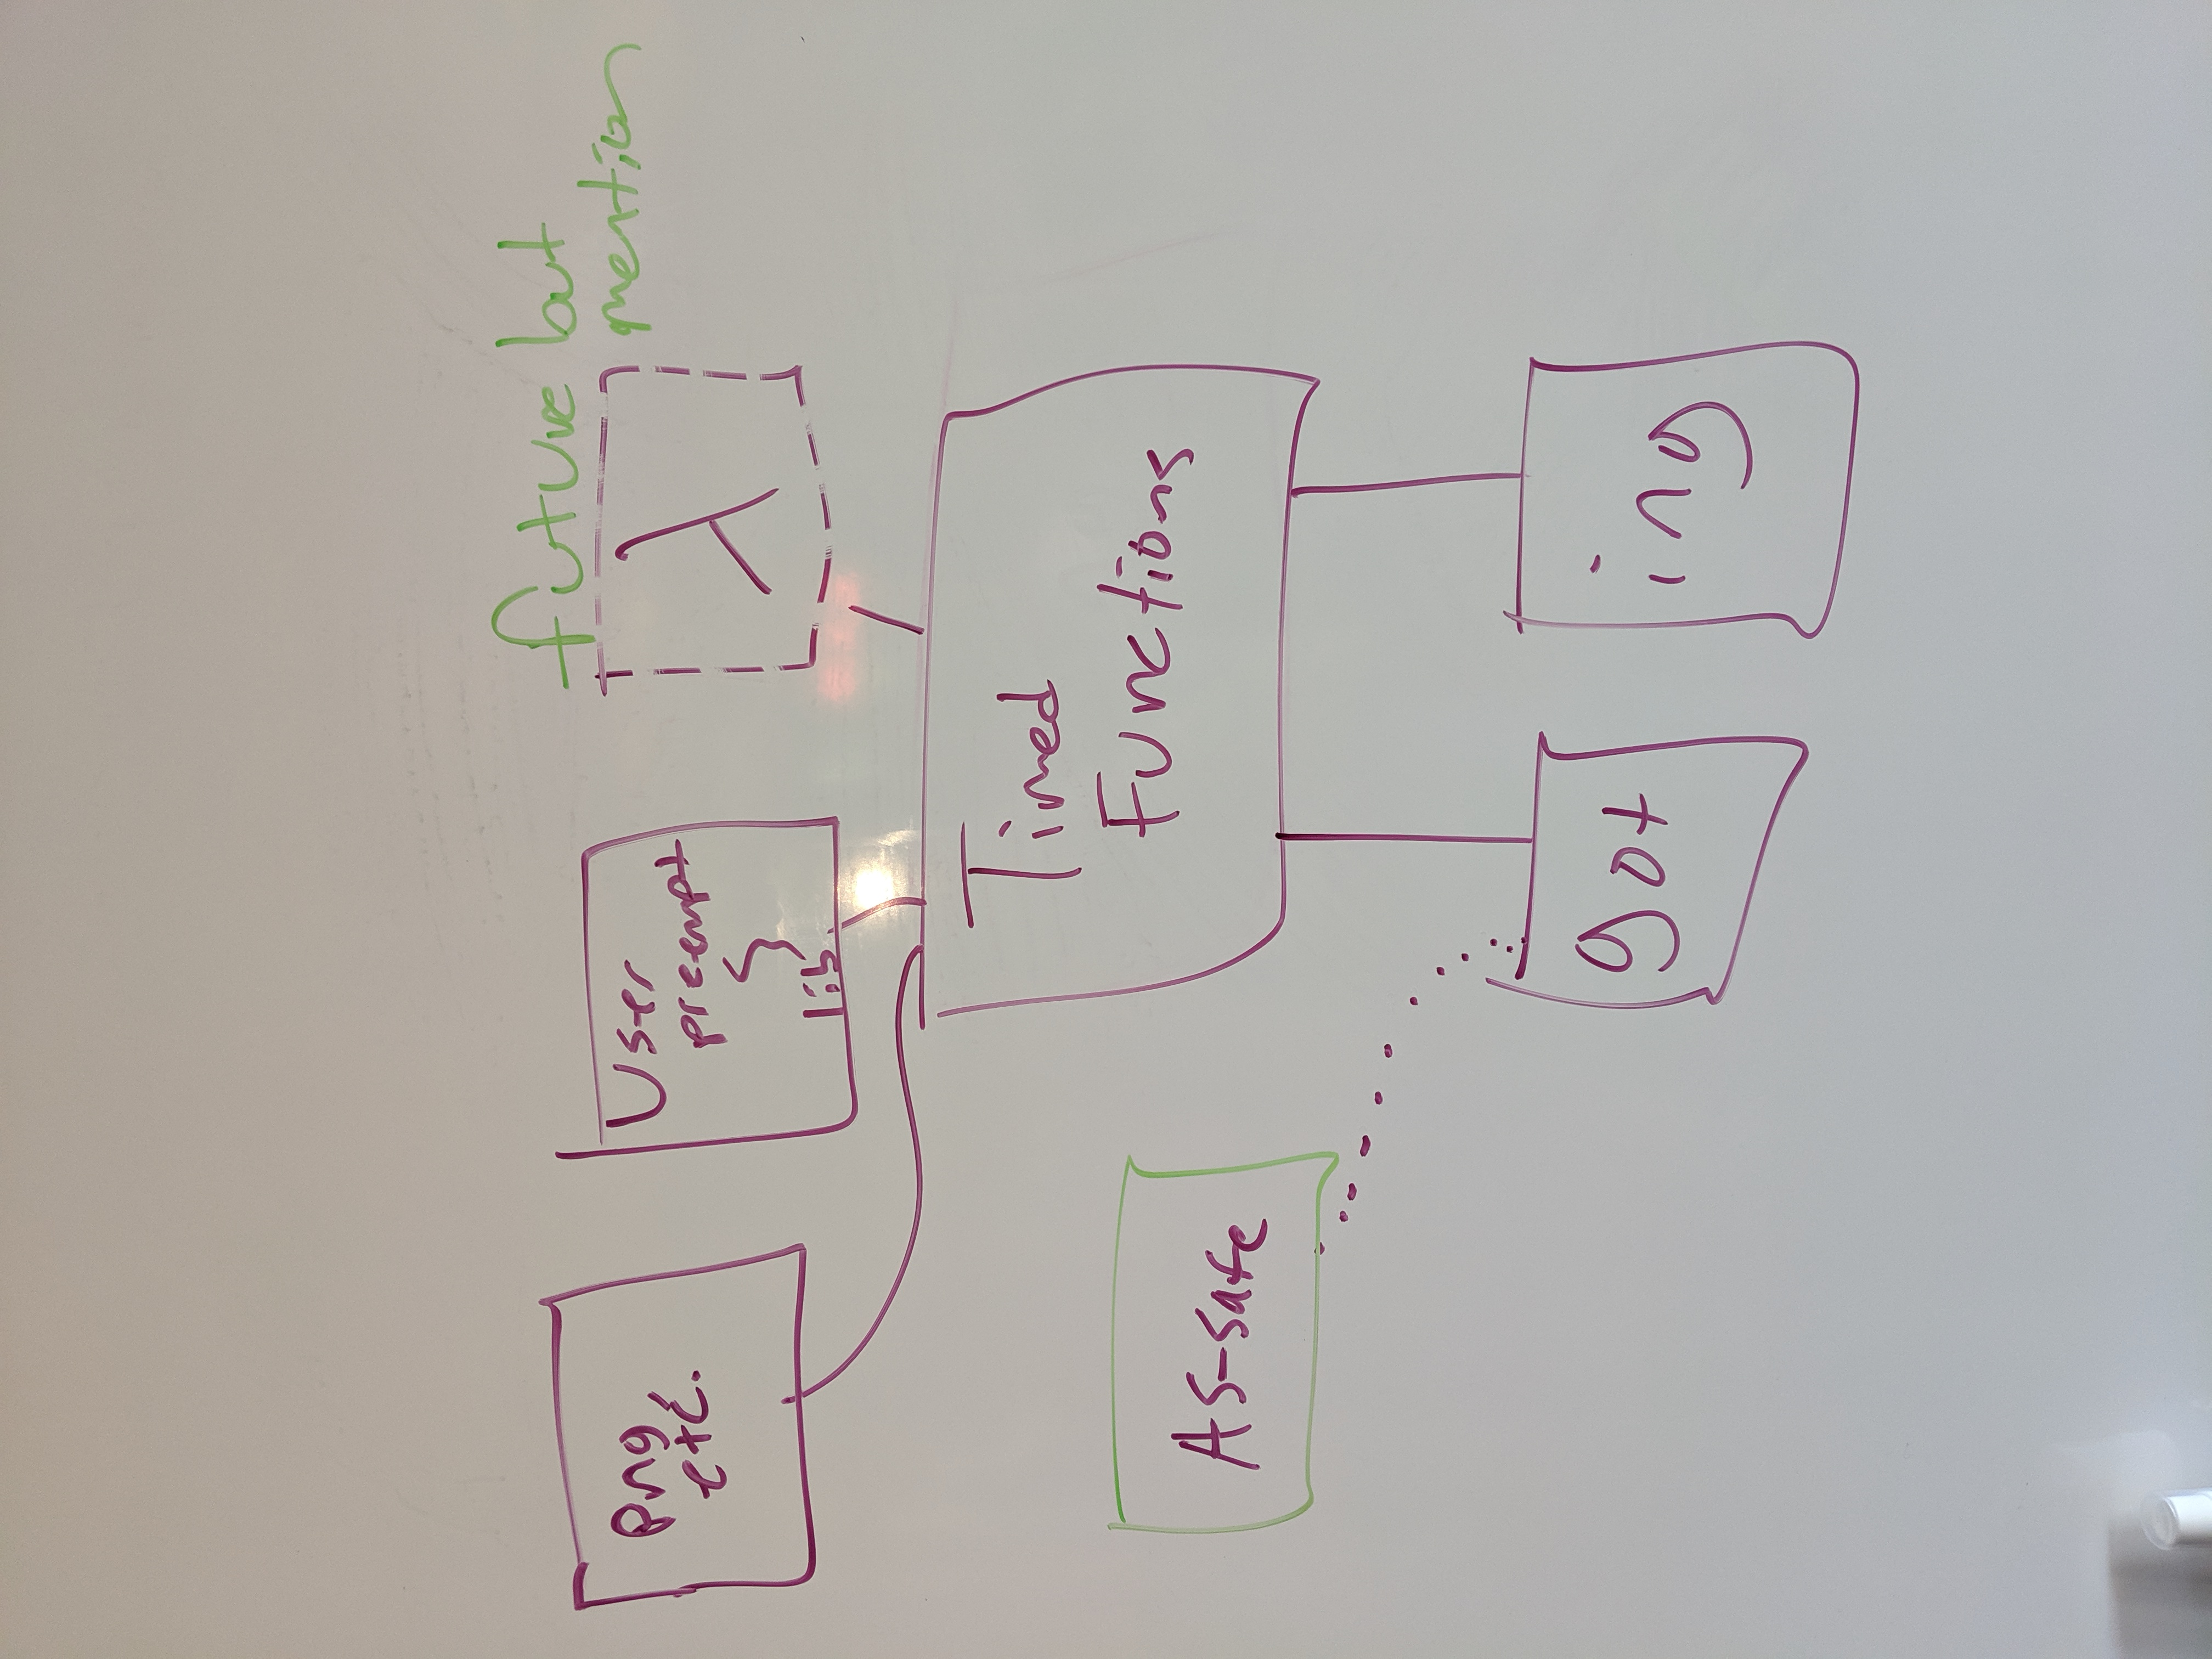
\includegraphics[width=0.75\columnwidth]{figs/architecture}
\end{center}
\caption{The preemptible functions software stack.  \textnormal{Rectangular boxes
represent components implementing the preemptible functions abstraction.  Ovals
represent components built on top of these.  Hexagonal boxes show the
required runtime environment.}}
\label{fig:architecture}
\end{figure}


\subsection{Automatic handling of shared state}

As we found in Section~\ref{sec:intro}, a key design challenge facing
\textit{libinger} is the shared state problem:  Suppose a preemptible function
$\mathcal{F}_0$ calls a stateful routine in a third-party library $\mathcal{L}$, and
that $\mathcal{F}_0$ times out and is preempted by \textit{libinger}.  Later, the
user invokes another timed function $\mathcal{F}_0'$, which also calls a stateful
routine in $\mathcal{L}$.  This constituting a concurrency violation,
\textit{libinger} must hide state modifications in $\mathcal{L}$ by $\mathcal{F}_0$
from the execution of $\mathcal{F}_0'$ to avoid undefined behavior.

The problem is actually even worse.  Those familiar with POSIX signals may notice
that, upon a function's timeout, its caller interrupts it.  \textit{The rest of the
program} can therefore be viewed as a signal handler, and would normally be expected
to restrict itself to calling async-signal-safe (roughly, nonreentrant)
functions~\cite{signal-safety-manpage}.

One non-solution to this problem is to instead prevent preemptible functions from
calling into third-party code (Section~\ref{sec:related}), but doing so would
severely limit their usefulness.  Instead, our approach
is to automatically and dynamically create copies of $\mathcal{L}$ to
isolate state from different timed functions.  Making this work on top of
existing systems software required solving many
design and implementation challenges, which we cover when we introduce
\textit{libgotcha} in Section~\ref{sec:libgotcha}.

\solb{Mention the concurrency implications of the API, and their relation to Rust's
safety guarantees.}


\subsection{Execution stacks}

Recall that, when a preemptible function times out, \textit{libinger} returns a
continuation object.  The caller might pass this object around the program, which
could later call \texttt{resume()} from a different stack frame.  Thus, the
continuation must contain not only the register context, but also the stack
frames belonging to the preemptible function and its callees.  The \texttt{launch()}
function enables this by switching to a new, dedicated stack just before invoking the
user-provided function.

Because of the infeasibility of moving these stacks after a function has started
executing, \textit{libinger} currently heap-allocates large 2-MB stacks so it can
treat them as having fixed size.  The latency of performing these large allocations
was once responsible for an order of magnitude increase in the time overhead of the
\texttt{launch()} operation, so \textit{libinger} now preallocates a large pool of
reusable stacks the first time it is used.


\subsection{Timer interrupts}

\begin{figure}
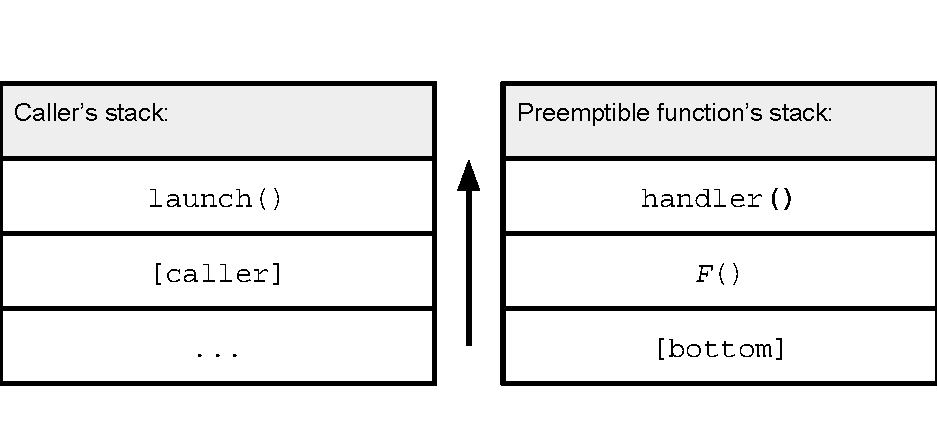
\includegraphics[width=\columnwidth]{figs/twostacks}
\caption{The stacks before and after a timeout.  \textnormal{Upon discovering
that the preemptible function has exceeded its time bound, the handler jumps into the
\texttt{launch()} function.  Then, \texttt{launch()} returns to the original call
site, removing its stack frame in the process.}}
\solb{Remove the continuations from this diagram and add the handler's stack frame.}
\label{fig:twostacks}
\end{figure}

Whenever \textit{libinger} is executing a user-provided function, we
enable fine-grained timer interrupts to
monitor that function's elapsed running time.  A timer interrupt fires
periodically, causing our signal
handler to be invoked each time.  If the function exceeds its timeout,
this handler saves a continuation by dumping the machine's registers.  It then
performs an unstructured jump out of the signal handler and back into the
\texttt{launch()} or \texttt{resume()} function, switching stacks as it does so.
Figure~\ref{fig:twostacks} shows the two stacks of execution
that are present while the
signal handler is running.

A subsequent \texttt{resume()} call restores the registers from the stored
continuation, thereby jumping back into the signal handler.  The handler
returns, resuming the preemptible function from the instruction that was executing
when the preemption signal arrived.

For simplicity, we use a fixed signal frequency for all preemptible
functions, but this is not fundamental to the design.  In the future, we plan to
adjust each function's frequency based on its timeout, and to delay the first signal
until
shortly before the time limit (in the case of longer-running functions).

\solb{THESIS: Removed discussion of our signal pool trick for notifying specific
POSIX threads.}

\solb{THESIS: Removed discussion of our self-signaling trick for restoring a signal
handler's POSIX context without using \texttt{setcontext()}.}


\subsection{Cancellation}

Should a caller decide not to finish running a timed-out preemptible function, it
must deallocate it.  In Rust this happens implicitly via the \texttt{linger\_t}
type's destructor, whereas users of the C interface are responsible for explicitly
calling the \textit{libinger} \texttt{cancel()} function.

Cancellation cleans up the \textit{libinger} resources allocated by
\texttt{launch()};
however, the current implementation
does not automatically release resources already claimed by the
preemptible function itself.  While the lack of a standard resource deallocation API
makes this inherently hard to do in C, it is possible in languages
such as Rust that support destructors.  For instance, the approach proposed by
Boucher et al.~\cite{boucher:atc2018} could be employed to raise a panic
(exception) on the preemptible function's stack.  This in turn would cause the
language runtime
to unwind each stack frame, invoking local variables' destructors in
the process.


\subsection{Performance goals}

\solb{Does any of this section belong in the Evaluation, Future Work, or Conclusion?}

Unlike prior work on low-latency preemptive scheduling such as
Shinjuku~\cite{Kaffes:nsdi2019}, \textit{libinger} runs on top of the existing
OS.  An obvious design to achieve this goal would be to use a thread or a process,
and although we argued in Section~\ref{sec:intro} that such an implementation would
still be far from trivial, our avoidance of these mechanisms has as much to do with
speed.  On Linux, simply spawning a thread incurs an order of magnitude more latency
than our \texttt{launch()} and \texttt{resume()} functions, and forking a process
costs an additional order of magnitude (Section~\ref{sec:eval}).

Recognizing that the asynchrony of interrupting a preemptible function does not imply
inherent asynchrony in accessing its result led us to develop a synchronous
abstraction, thereby obviating the need for the aforementioned spawn operations on
the critical path.  But we deliberately diverged from the design of Shinjuku and RT
in another way as well:\@ unlike these systems, we make each thread responsible for
its own preemption rather than serving preemption signals from a shared watchdog
thread.  This decision was informed by back-of-the-envelope calculations based on
Shinjuku's comparison of the end-to-end latency of bare-metal interprocessor
interrupts (IPIs) versus Linux signals.

While Shinjuku reports that IPIs take an average of only 1,993 cycles, compared to
4,950 for signals (roughly 1:2.5), their sender/receiver breakdown of the latter
number suggests significant latency savings by avoiding cross-core signaling:
First, 343 of those cycles (6.9\%) are spent propagating the signal between the two
cores; we expect this delay to be nearly absent for a timer interrupt originating at
its destination core's own local interrupt controller.  Second, 2,084 cycles (42\%)
are incurred by the sending core; assuming the interrupt controller supports
periodic timer interrupts at the necessary frequency, this cost does not need to be
paid between each interrupt, suggesting measurable savings here too.  Although
our prototype is not yet optimized to this extent, we expect it is possible for a
system built on intra-thread Linux signals to achieve an average preemption latency
within 2x that of Shinjuku's custom operating system.

Of course, in our design, increasing the accuracy of preemption is a tradeoff:\@ more
frequent timer signals mean a tighter bound on timeout detection, but also a lower
throughput of useful work.  The correct balance certainly depends at least on the
timeout value and size of the function, and merits further study.

\solb{THESIS: Could try to confirm these predicted measurements.}

\solb{THESIS: Could explore strategies for choosing POSIX timer intervals.}

\section{Thread library: \textit{libturquoise}}
\label{sec:libturquoise}

\textit{Shinjuku} observes that ``there have been several efforts to implement
efficient, user-space thread libraries.  They all focus on cooperative
scheduling''~\cite{Kaffes:nsdi2019}.  We agree that such libraries are rare, and
attribute this to a lack of natural abstractions to support them.  (Though
\textit{RT} from Section~\ref{sec:related} could be a counterexample, its lack of
nonreentrancy support makes it far from general purpose.)

While the preemptible function is a fundamentally synchronous abstraction, its
simplicity makes it readily composable, and indeed, well-suited to implementing
preemptive threading.  As a proof of concept, we have created a
preemptively-scheduled userland thread library, \textit{libturquoise}\footnote{so
called because it implements ``green threading with a twist''}, by modifying the
\textit{tokio-threadpool}~\cite{www-tokio-threadpool} work-stealing scheduler from
the Rust futures ecosystem.

To migrate the thread pool workers to preemptive scheduling, we made them poll each
task future from within a preemptible function.  We did this in
just 120 new lines of Rust, 50 of them added to version 0.1.16 of the thread library
and
70 spent augmenting \textit{libinger}'s Rust API with a reusable \textbf{preemptible
futures} adapter.

Currently, \textit{libturquoise} assigns each future it launches or resumes the same
fixed time budget, although this design could be extended to support
multiple job priorities.  When a task times out, the scheduler pops it from its
worker thread's job queue and pushes it onto the incoming work queue,
offering it to any available worker for rescheduling after all other waiting jobs
have had a turn.


\subsection{Preemptible futures}

For seamless interoperation between preemptible functions and the futures ecosystem,
we built a preemptible future adapter that wraps the \textit{libinger} API.  This
can be used to pass preemptible functions into a platform designed to process
futures.

Because
of languages' differing futures, this integration is not portable like the core API.
Fortunately, its implementation is a straightforward application of
\texttt{pause()} to propagate cooperative yields across the preemptive function
boundary:\@ we present the general construction of the preemptible future
type and an algorithm for polling one in Listing~\ref{lst:future}.

\begin{figure}
\begin{lstlisting}[label=lst:future,caption=Futures adapter type (pseudocode)]
function PreemptibleFuture(Future fut,
                              Num timeout):
  function adapt():
    while poll(fut) == NotReady:
      pause()
  fut.linger = launch(adapt, 0)
  fut.timeout = timeout
  return fut

function poll(PreemptibleFuture fut):
  resume(fut.linger, fut.timeout);
  if has_finished(fut.linger):
    return Ready
  else
    if called_pause(fut.linger):
      notify_unblocked(fut.subscribers)
    return NotReady
\end{lstlisting}
\end{figure}

\chapter{Nonreentrancy and selective relinking: \\ the \textit{libgotcha} runtime}
\label{chap:libgotcha}

\ifdefined\chapquotes
\vspace{-1in}
\begin{chapquote}[1.5in]{James S.\@ A.\@ Corey, \textit{Nemesis Games}}
`Alien superweapons were used,' Alex said, walking into the room, \\
sleep-sweaty hair standing out from his skull in every direction. \\
`The laws of physics were altered, mistakes were made.'
\end{chapquote}
\fi

In Section~\ref{sec:libinger:reentrancy}, we saw that it is not safe in general for a
preemptible function to call into stateful code that was written without the
preemptible function abstraction in mind.  However, such code is prolific in the
modern systems stack, and in order to support interoperability with it, we need to
automatically transform the program to fix the safety hole.  This chapter covers a
novel software system designed to do just that, dubbed \textit{libgotcha}.

\begin{figure}
\begin{center}
\includegraphics[width=0.7\columnwidth]{figs/procimg_perobj}
\end{center}
\caption{Layout of a typical module within the process image.  \textbf{Bold} sections
contain program data; \textit{italicized} ones contain metadata for the runtime.}
\label{fig:procimgobj}
\end{figure}

\begin{promotesubsections}
\begin{swallowsections}
\input[functions]{gotcha_gotcha}
\end{swallowsections}
\end{promotesubsections}
\hspace{-2.5em}
Our discussion in this chapter uses \textit{libinger} as a motivating example of a
\textit{libgotcha} user, as this configuration was the inspiration for the runtime's
creation.  However, we have found that the described techniques to be general and
equally relevant to applications besides timed functions.  As such,
\textit{libgotcha} exposes a general API that allows any \textbf{control library} to
configure its behavior for the process.  We give more details later in the chapter,
and study other examples of control libraries in Chapter~\ref{chap:safety}.


\section{A brief tour of linking}
\label{sec:libgotcha:link}

We begin with background about linking, a two-stage process that ultimately produces
an in-memory \textbf{process image} containing a program's code, all the data it
needs to execute, and the code and data of all its dependencies.  Linking operates on
\textbf{object files} that can take the form of either an \textbf{executable} or a
\textbf{shared library}.  Once a program is running, its process image contains a
region corresponding to each loaded object file.  We will refer to each such region as
a \textbf{module}, regardless of whether it corresponds to an executable or a shared
library.  Each module is divided into logical \textbf{sections}, each containing a
particular type of information.  Figure~\ref{fig:procimgobj} shows a typical module's
layout; notice that it contains both data corresponding to the source code and
generated metadata for runtime consumption.

The linking process occurs in two parts.  Static linking occurs at compile time and
forms the last step of the traditional build process.  Dynamic linking occurs at a
phase of runtime we will refer to as \textbf{load time}, because it starts before the
program has been loaded from disk or the language runtime initialized.


\subsection{Static linking}

Invoking the \texttt{cc} compiler driver does more than just compile C code:\@ it
runs the C preprocessor \texttt{cpp}, the C compiler (\texttt{cc1} in GCC's case),
then the static linker \texttt{ld}.

The output of the second step is a relocatable object file containing code and data
with referenced addresses identified by named \textbf{symbols}.  In a relocatable
object file, symbol \textbf{references} such as instructions making function calls
or accessing global variables are encoded with a null address as a placeholder.  Each
object file contains a \textbf{relocation table} in a separate section that
associates each placeholder with a symbol name, which may or may not be located in
the same file.  Each object file also contains a \textbf{symbol table} to identify
the symbols it defines and associate them with the file offset of their definition.
Note that only non-\texttt{static} C symbols generate global symbol table entries
that can be referenced from other object files; this keyword is confusingly named and
does not refer to static linking.  The compiler's ultimate output is one relocatable
object file for each source file.

The static linker is responsible for combining one or more relocatable object files
into a single executable or shared library, where either type of output file is
ready for loading into memory for execution.  This process consists of verifying that
there is a definition corresponding to each symbol reference, unifying the sections
across object files and choosing a final address (or relative address) for each
symbol, encoding the chosen addresses at the location recorded in each relocation
table entry, and writing the resulting file to disk.  This output file does not
preserve the relocation table because the linker has already fixed the null pointers
it described.  The file does contain a symbol table because it can be useful for
debugging (e.g., to generate stack traces), but this can be removed using the
\texttt{strip} utility without affecting the program semantics.

With the exception of macOS, most modern Unix systems use ELF (Executable and
Linkable Format) object files.  One advantage of this format is that executables and
shared libraries are themselves ELF object files.


\subsection{Dynamic linking}
\label{sec:libgotcha:dylink}

Static linking allows programs to reuse ``libraries'' of precompiled object files,
but each program must be built with its own copy of all its libraries within the
executable.  This means that every time an application is loaded, its libraries' code
and data must be read back from disk, even if another running program uses the same
libraries; it also means that updating a library requires recompiling all dependent
programs installed on the system.  Dynamic linking solves both problems by separating
libraries into separate files that are not read until the executable runs.\footnote{
Specifically, this separation obviates the need to read the files from disk multiple
times because the runtime maps them into the process image using the \texttt{mmap()}
family of system calls.  The kernel tracks regions that are already mapped and serves
recurring requests from memory instead of disk, mapping to the same physical memory
if the pages are read-only or creating copy-on-write page mappings otherwise.}

By splitting libraries into their own files, dynamic linking introduces a build-time
challenge:\@ the relative position and offset of modules cannot be known until
runtime.  As such, rather than performing the relocations for inter-module symbol
references, the static linker leaves the placeholder addresses and adds a separate
dynamic relocation table and dynamic symbol table into the output object file.
Unlike the tables used for static linking, these are needed to launch the program, so
tools such as \texttt{strip} leave them in place.  For executables, the linker also
writes the path to an ``interpreter'' program into the ELF program header.

When asked to load a program that declares an interpreter, the kernel loads and jumps
to the interpreter instead of the executed program.  Usually, this interpreter is the
system \textbf{dynamic linker}, traditionally named \texttt{ld.so}.  Before jumping
into the program code, the dynamic linker loads all the modules and processes the
entries in each of their dynamic relocation tables.  The relocations are not
restricted to modifying writeable memory:\@ they can update constant global data and
even executable instructions.  Even if they leave the code unchanged, its position
relative to the rest of the module matters.  These points are critical to our use
case, as they mean that in order to duplicate modules' data, we must also duplicate
their code.

Another consequence of relocations being able to alter read-only memory is that the
dynamic linker must change the page protections of these regions after it is finished
processing relocations.  To support this, the compiler splits up module components
into fine-grained sections by purpose.  Non-\texttt{const} global variables are
placed in the \texttt{.data} and \texttt{.bss} sections, which must remain writeable
at runtime and therefore require no special action.  In contrast, \texttt{const}
globals are split between the \texttt{.rodata} and \texttt{.data.rel.ro} sections
based on whether they require relocation; in the latter case, the dynamic linker
marks the pages read-only before passing control to the program.

If relocations routinely modified scattered locations throughout the executable
\texttt{.text} section, the dynamic linker would have to change page protections on
most or all of each module's code pages.  This would require a lot of system calls,
but it would also require copy-on-write code mappings, preventing instruction cache
hits between processes using the same library.  To avoid these problems, the compiler
indirects references to dynamic symbols via a structure called the GOT (Global Offset
Table).

\begin{figure*}
\begin{minipage}{\textwidth}
	\includegraphics[width=\textwidth]{figs/gotables-crop}
	\subcaption{Reading a library's global variable: \texttt{size\_t tmp = data;}}
	\label{fig:dytabs:got}
	\end{minipage}

	\begin{minipage}{\textwidth}
	\includegraphics[width=\textwidth]{figs/pltables-crop}
	\subcaption{Calling an eagerly-resolved library function: \texttt{fun()}}
	\label{fig:dytabs:plt}
	\end{minipage}

	\begin{minipage}{\textwidth}
	\includegraphics[width=\textwidth]{figs/jstables-crop}
	\subcaption{Calling a lazily-resolved library function.  In step \textcircled{5},
	the dynamic linker memoizes the resolved address into the GOT; subsequent calls
	proceed as above.}
	\label{fig:dytabs:lazy}
	\end{minipage}
\caption{Table references required to reference global symbols in dynamically-linked
programs}
\label{fig:dytabs}
\end{figure*}

The GOT is a table of relocated pointers to symbol definitions, whether those
definitions are within the same module or in a different one.  To avoid generating
code pages that require relocations, the compiler compiles each reference to or
dereference of non-\texttt{static} global data into a position-independent load of
the corresponding pointer from the GOT.  Figure~\ref{fig:dytabs:got} shows an example
of the two instructions and one table reference needed for a dereference.  A
reference would generate only the first \texttt{mov} instruction, as would taking a
pointer to a function.

Calling a global function works differently and relies on another indirection
structure called the PLT (Procedure Linkage Table), which contains code instead of
pointers.  For each call to a non-\texttt{static} function, the compiler generates a
position-independent call to a PLT entry corresponding to the function being called.
It generates a PLT entry, which is a short sequence of instructions that loads the
pointer to the real definition from the GOT, then executes and indirect jump to that
location.  Figure~\ref{fig:dytabs:plt} shows an example function call.  As with GOT
entries, there are PLT entries for functions defined both within and outside the
referencing module.

Not all function calls are this simple.  To save the dynamic linker some work at load
time, many function calls resolve lazily on their first execution.  Such resolution
involves a series of jumps designed to memoize the address so that subsequent calls
to the function from the same module do not repeat the expensive lookup.
Figure~\ref{fig:dytabs:lazy} shows the effect of the first call to such a
function:\footnote{This representation is slightly simplified for brevity.  In
practice, it is undesirable to hardcode the address of a dynamic linker function into
each module.  Therefore, instead of jumping directly to the symbol resolver, the slow
lookup path jumps to a dedicated PLT stub that loads its address from another GOT
entry.  Technically, there are separate identifiers for the symbol and the module,
each pushed to the stack by one of these two involved PLT stubs.}  \textcircled{1}
The program calls the PLT stub, just as it would for an eagerly-resolved function.
\textcircled{2} The PLT stub is longer (three instructions instead of one), but still
begins with an indirect jump to the pointer found in the corresponding GOT entry.
\textcircled{3} The GOT entry initially contains the address of the PLT stub's second
instruction, so the indirect jump is a no-op and merely advances the instruction
pointer.  \textcircled{4} The rest of the PLT stub pushes a constant identifying the
module and symbol onto the stack, then jumps to a symbol-lookup function in the
dynamic linker.  \textcircled{5} After looking up the address of the symbol's
definition, the dynamic linker uses the identifier from the stack to find and update
the GOT entry in the calling module.  \textcircled{6} The dynamic linker jumps to the
symbol in the defining module.  Because the GOT entry has been updated, future calls
proceed exactly like eagerly-resolved ones and jump directly to the symbol definition
from the first instruction of the PLT stub.  Of course, the GOT entries associated
with lazy PLT stubs must be writeable at runtime; this is why
Figure~\ref{fig:procimgobj} shows the GOT as split between two sections.

The dynamic linker performs all relocations and other standard module setup
automatically at load time, but the initialization process is pluggable.  In
particular, modules can include \textbf{constructor} functions to be invoked before
control is transferred to the runtime and ultimately the program's main function.  As
we will see, our work leverages this feature to override certain relocations at the
conclusion of load time.


\begin{promotesubsections}
\begin{swallowsections}
\input[functions]{gotcha_namespaces}


\input[functions]{gotcha_libsets}

Thus, selective relinking is selective in two ways, only affecting execution when the
next libset differs from the current libset and the program references a dynamic
symbol defined in a module that is not currently executing on that thread.

\solb{Expand interface listing and add comments with section references}
\end{swallowsections}
\end{promotesubsections}


\subsection{Detecting cross-module symbol references}

Identifying which GOT entries correspond to cross-module symbol references is a
multi-step process:
First, we traverse the relocation table for each loaded module, cross referencing
each of its relocation entries against the local module's symbol table.  If the
symbol table does not contain a definition matching the relocation entry's target, we
conclude that the relocation must correspond to a cross-module call.  Otherwise, we
check the address in the GOT entry corresponding to the relocation:  If this address
is outside the memory bounds of the current module, it is a cross-module call.
Otherwise, if this address matches the one from the symbol table entry, it is not a
cross-module call, and should be skipped.  The trickiest case is when the GOT entry
does not match but does point somewhere within the current module, since this means
it probably still refers to the PLT stub (because the symbol reference is lazy and
has not yet been resolved, as covered at the end of
Section~\ref{sec:libgotcha:dylink}).  In this case, we resolve the symbol early,
update the GOT entry, and recheck whether it resolved to the local definition to
determine whether it is a cross-module call.


\begin{promotesubsections}
\begin{swallowsections}
\input[functions]{gotcha_init}
\end{swallowsections}
\end{promotesubsections}

If a preemptible function is canceled rather than being allowed to return, execution
might be interrupted within a call to a library function.  For this reason,
\textit{libgotcha} must treat the libset's shared state as corrupted; it provides the
\texttt{libset\_reinit()} function shown in Listing~\ref{lst:gotchaapi} to allow
control libraries to inform it of such a situation so it can \textbf{reinitialize}
the libset before returning it to the pool.

Our early approach to reinitialization was to unload and reload all objects in the
libset by calling \texttt{dlclose()} followed by \texttt{dlmopen()}.  While this
approach theoretically allowed us to delegate the work to the dynamic linker, in
practice it introduced significant complications.\footnote{Most notably, some shared
libraries are marked with a special configuration flag, \texttt{DF\_1\_NODELETE},
which prevents the dynamic linker from ever removing them once they have been loaded.
Because almost all libraries depend on libc, the presence of even one such library
would prevent us from reinitializing a libset.  The flag is mostly used on libraries
that need to monkey-patch some other loaded library, such that the two subsequently
have a circular dependency.  Fortunately, this was not generally a problem for us
because when we unload one library from a libset, we then unload the rest.  Whenever
we encountered a \texttt{NODELETE} object file, we would make a special copy with the
flag cleared, for loading into every namespace except the main one.}  Worse, it
required the dynamic linker to reprocess all relocations throughout the libset, which
introduced prohibitive runtime latency.  We measured reinitialization taking almost 5
ms (over 10 million cycles on modern processors) on even small minimal example
programs~\cite{boucher:atc2020}.  With such delays, the only reasonable way for the
control library to handle cancellation was to delegate the reinitialization to a
separate thread to take it off the critical path; of course, this approach only works
as long as the number of libsets is not a bottleneck.

We have since redesigned reinitialization around a significantly faster approach:\@
checkpointing only portions of each module.  The key insight is that, as we saw in
Section~\ref{sec:libgotcha:link}, only some sections are writeable at runtime.  We
can therefore assume that these are the only memory regions of each module that can
change.  After populating the libset pool at application start, \textit{libgotcha}
iterates through each module of each libset and makes a backup copy of all its
writeable regions.  When a control library calls \texttt{libset\_reinit()},
\textit{libgotcha} restores each such region from the backup before returning the
affected libset to the pool.  We summarize this approach, which has reduced the
latency of reinitialization by two orders of magnitude, in
Figure~\ref{fig:reinit}.\footnote{We will address the version watermark alluded to
therein later in this chapter.}  To avoid having to repeat relocations and rerun any
module constructors, we capture the backup after dynamic relocation is complete and
all constructors have run; the tradeoff is that we actually have to copy memory,
rather than leveraging copy on write to later restore to the version on disk.

\begin{figure}
\includegraphics[width=\columnwidth]{figs/reinit-crop}
\caption{Libset reinitialization to support asynchronous cancellation}
\label{fig:reinit}
\end{figure}


\section{Selective relinking}

Most of the complexity of \textit{libgotcha} lies in the implementation of selective
relinking, the mechanism underlying libset switches.  To establish the libset
abstraction, it must arrange to conditionally intercept cross-module symbol
uses based on the currently-configured next libset.

As we saw in Section~\ref{sec:libgotcha:dylink}, whenever a program references a
dynamic symbol, it looks up the address of the definition in a data structure called
the global offset table (GOT).  Selective relinking works by shadowing the
GOT.\footnote{Hence the name \textit{lib\textbf{got}cha}.}  Just after the dynamic
linker populates the GOTs, \textit{libgotcha} replaces every entry that should
sometimes trigger a libset switch with a fake address.  It stores the original
address in its shadow GOT, which is organized by the libset that houses the
definition.  The fake address used depends upon the type of symbol:


\subsection{Intercepting function calls}

When setting up selective relinking, we do not know whether a particular function
call needs to be rerouted until runtime.  However, the fact that dynamic function
calls consult the GOT to determine which code to execute makes it efficient and
relatively straightforward to receive a notification whenever they occur.  To set
this up, at load time, we replace each such cross-module GOT entry with the address
of the special \textit{libgotcha} function \texttt{procedure\_linkage\_override()}.
Whenever the program tries to call one of the affected functions, control transfers
to this function instead; it then checks the thread's next libset, looks up the
appropriate symbol definition in the shadow GOT, and jumps to that location.  Because
\texttt{procedure\_linkage\_override()} runs between the caller's \texttt{call}
instruction and the real function, it is written in assembly to avoid clobbering
registers (e.g., those used for argument passing).

There is one major complication that necessitates an additional level of indirection
beyond what we have described.  Recall from the eagerly-resolved function calling
sequence in Figure~\ref{fig:dytabs:plt} that each function call site calls a
one-instruction PLT stub that performs an indirect jump to the real definition via
the GOT.  This means that if we simply replaced all the GOT entries with the address
of \texttt{procedure\_linkage\_override()}, that function would not know which GOT
entry it was being called via, and therefore which symbol to look up.  Instead, we
introduce our own table of executable stubs called the PLOT (Procedure Linkage
Override Table).  Unlike PLT entries, ours always push an identifier indicating which
function is being called.  For this, we use indices into a custom data structure
called the GOOT (Global Offset Override Table), which stores enough information to
find the symbol's shadow GOT entries while being practical to traverse in handwritten
assembly code.  Figure~\ref{fig:override} summarizes the modified dynamic function
call sequence under selective relinking.

\begin{figure}
\includegraphics[width=\textwidth]{figs/tables-crop}
\caption{Calling an eagerly-resolved library function under selective relinking}
\label{fig:override}
\end{figure}

A subtle but important point about dynamic linking is that pointers to the same
definition must compare equal, regardless of where they are obtained.  For instance,
the reader might notice that invocation is not the only thing a program can do with a
function:\@ it might also pass around the function's address.  In fact, after taking
the address, it could pass it to code within a different module, which might need to
know whether a third module passed a pointer to the same function.  To support such
comparisons, the compiler exclusively generates eagerly-resolved relocations for any
function that a particular module obtains a pointer to.  This way, the \texttt{mov}
to retrieve the pointer always finds the resolved address of the real definition in
the GOT.  To avoid breaking pointer comparison, \textit{libgotcha} associates each
PLOT entry with its function's definition, not its call site or calling module.  This
provides correct comparison semantics because all references to a particular function
receive the same pointer to a particular PLOT entry, and although this pointer
technically refers to the corresponding symbol's definitions in all libsets, at any
one time all calls to it will only resolve to the definition in the next libset.
Since at any given time there can only be one next libset, calls to pointers that
compare equal always refer to the same copy of the definition.

The setup described so far works for eagerly-resolved function calls.  However,
recall that some function calls resolve to their definition lazily at runtime.  For
such calls, the dynamic linker memoizes the resolved address by updating the GOT
entry, as shown in Figure~\ref{fig:dytabs:lazy}.  Unfortunately, replacing this GOT
entry would overwrite the PLOT pointer installed by \textit{libgotcha} at load time,
thereby preventing it from intercepting future calls to the function.  The write to
the GOT happens within the symbol-lookup code in the dynamic linker, so there is no
way to skip it.  Luckily, the dynamic linker keeps each module's dynamic relocation
table in memory and uses that to determine which GOT entry to update.  The
\textit{libgotcha} constructor exploits this by marking the relocation table pages
writeable, changing the relocation entries corresponding to cross-library calls, then
restoring the protection bits.  This fools the dynamic linker's lazy symbol lookup
into later updating the shadow GOT entry instead.  Not only does this avoid breaking
selective relinking, it also preserves memoization.


\subsection{Intercepting global variable accesses}

\begin{promotesubsections}
\begin{swallowsections}
\input[functions]{gotcha_globals}

\solb{\textbf{Subsection on thread-local storage}}

\solb{Diagram of thread-local data layout}

\solb{Reinitialization diagram (TLS part)}


\input[functions]{gotcha_uncopyable}

\solb{Add the effects in the above TODO to the UML diagram?}

\solb{Stipulate that libgotcha itself is always uncopyable}

\solb{Say that the hook function runs in the interrupted module's namespace}

\solb{Mention pre-call hooks}

\solb{Give the limitations of each type of hook}

\solb{\textbf{Section More on control libraries}}

\solb{Types of control libraries from the frontmatter}

\solb{Address monomorphization}

\solb{Monkey patching of ld.so and library header rewriting trick}


\input[functions]{gotcha_tls}

\solb{Drop TLS stuff, incorporating whatever is salvageable earlier}

\input[functions]{gotcha_linker}

\solb{Recompiling glibc from the frontmatter}

\input[functions]{gotcha_relocations}

\end{swallowsections}
\end{promotesubsections}


\section{Evaluation}

\input[functions]{eval_ugotcha}

\input[functions]{eval_testbed}

\solb{Thread creation, TLS allocation, and libtlsblock}

\section{Deployment}
\label{sec:deploy}

We now describe our microservices in the broader context of our full proposed
serverless system.  We clarify their lifecycle, interactions with the compute nodes,
and the trust model for the cloud provider.

Users submit their microservices in the form of Rust source code, allowing the
serverless operator to pass the \texttt{-Funsafe-code} compilation flag to reject
any \texttt{unsafe} code.  This process need not occur on the compute
nodes, provided the deployment server tasked with compilation runs the same version
of the Rust compiler\footnote{This restriction exists because, as of the latest
release (1.23.0) of the compiler, Rust does not have a stable ABI.}.  The operator
needs to trust the compiler, standard library, and any libraries against which it
will permit the microservice to link (since they might contain \texttt{unsafe} code),
but importantly need not worry about the microservice itself.

We believe that many users would find it acceptable to be presented with a specific
list of permitted dependencies.  But how big a list could the provider hope to offer
at the time of launching the service?  It bears noting that libraries including only
safe Rust code could be whitelisted without review.  To approximate how big such a
list would be given the current Rust ecosystem, we turn to a 2017
study~\cite{www-cratesio-unsafe} by the Tock authors that found just under half of
the Rust package manager's top 1000 most-downloaded libraries to be free of
\texttt{unsafe} code.  They caution that many of those packages have unsafe
dependencies, but we suspect that reviewing a relatively small number of popular
libraries would open up the majority of the most popular packages.

If the application compiles (is proven memory-safe) and links (depends only on
trusted libraries) successfully, the deployment server produces a shared object file,
which the provider then distributes to each compute node on which it might run.
Then, in order to ensure that invokers will experience the warm-start latencies
discussed in Section~\ref{sec:motive}, those nodes' host processes should instruct
one or more of their workers to preload the dynamic library.  If the provider
experiences too many active microservices for its available resources, it can
unload some libraries; on their next invocation, they will experience higher
(cold start) invocation latencies since we need to synchronously load the dynamic
library.  In our measurements, the overhead of this operation is about 100\textmu{}s.

\section{Future work}

\solb{This isn't exactly a future work section, is it...?}

Like \textit{Shinjuku} and \textit{RT} before us, we have arrived at a preemptive
thread library; however, we have done so by building parallelism on top of
not the other way around.  Because of this, we have a more flexible abstraction, and
we intend to continue applying it to other problems.

\solb{Mention other use cases, such as the continuation-memoizing RPC server?}

But we have also diverged from \textit{Shinjuku} and \textit{RT}
in another way:\@ unlike these systems, we make each thread responsible for
its own preemption rather than serving preemption signals from a shared watchdog
thread.  This decision was informed by back-of-the-envelope calculations based on
Shinjuku's comparison of the end-to-end latency of bare-metal interprocessor
interrupts (IPIs) versus Linux signals.

While Shinjuku reports that IPIs take an average of only 1,993 cycles, compared to
4,950 for signals (roughly 1:2.5), their sender/receiver breakdown of the latter
number suggests significant latency savings by avoiding cross-core signaling:
First, 343 of those cycles (6.9\%) are spent propagating the signal between the two
cores; we expect this delay to be nearly absent for a timer interrupt originating at
its destination core's own local interrupt controller.  Second, 2,084 cycles (42\%)
are incurred by the sending core; assuming the interrupt controller supports
periodic timer interrupts at the necessary frequency, this cost does not need to be
paid between each interrupt, suggesting measurable savings here too.  Although
our prototype is not yet optimized to this extent, we expect it is possible for a
system built on intra-thread Linux signals to achieve an average preemption latency
within 2x that of Shinjuku's custom operating system.  It is our hope that further
optimization of our system, including through the adoption of some of Shinjuku's
continuation optimizations, will allow us to meet this performance goal.

Of course, in our design, increasing the accuracy of preemption is a tradeoff:\@ more
frequent timer signals mean a tighter bound on timeout detection, but also a lower
throughput of useful work.  The correct balance certainly depends at least on the
timeout value and size of the function, and also merits further study.

\solb{THESIS: Might want to accelerate kernel signal handling?}

\solb{THESIS: Might want to support nested preemptible functions?}

\section{Conclusion}

We presented the lightweight preemptible function, a composable new abstraction
for invoking a function with a timeout.  This enabled us to build a first-in-class
preemptive userland thread library by implementing preemption atop a cooperative
scheduler, rather than the other way around.  Our evaluation shows that lightweight
preemptible functions have overheads of a few percent (lower than similar OS
primitives), yet enable new functionality.

We believe the lightweight preemptible function abstraction naturally supports
common features of large-scale systems.  For example:  An ad renderer might implement
graceful degradation by rendering frames of an animation in a preemptible function,
dropping unfinished ones to meet its SLO.  An RPC server might preserve work by
processing each request in a preemptible function and memoizing the continuations; if
a request timed out but was later retried by the client, the server could resume
executing it from where it left off.


%\vspace{-0.1in}
%\section*{Acknowledgments}
% Comments for people we need to ack in the final version

%% Bibliography
\setlength{\bibsep}{2pt plus 1pt}  % plus 1pt seems to avoid widows/orphans
\small 
% \footnotesize % SPACE
\bibliography{ref}
\bibliographystyle{abbrvnat}
%\bibliographystyle{abbrvnat_noaddr} % SPACE
%\theendnotes % ENDNOTES
}{% !onlyAbstract
}

%\appendix
%\input{appendix_sources}

\end{document}

% Local Variables:
% TeX-command-default: "LaTeX PDF"
% End:

